\documentclass{article}
\usepackage{graphicx} % 添加 graphicx 包
\usepackage{amsmath} % 添加 amsmath 包以支持数学公式
\usepackage{geometry} % 添加 geometry 包以调整页面布局
\usepackage{CJKutf8}
\usepackage{setspace} % 添加 setspace 包以调整行间距
\geometry{a4paper, margin=1in}

\begin{document}
\begin{CJK}{UTF8}{gbsn}
\begin{titlepage}
    \centering
    \vspace*{2cm}
    {\Huge \textbf{Lecture Notes on CS231N}}\\[1.5cm]
    {\Large Yiwei Chen}\\[0.5cm]
    \vfill
    
\includegraphics[width=0.4\textwidth]{images/school_badge.png}\\[1cm] % 确保路径正确
    {\large Zhejiang University}\\[1cm]
    {\large \today}
\end{titlepage}

\onehalfspacing % 设置行间距为 1.5 倍

\section*{Lecture 1: History of CV and Introduction to CNNs}
\begin{itemize}
    \item \textbf{ImageNet:} Annual competition for image classification, started in 2010.
    \item \textbf{Convolutional Neural Networks (CNNs):} Introduced by Yann LeCun in 1998, CNNs are a type of neural network designed for processing structured grid data, such as images. CNNs show great performance in image classification tasks.
\end{itemize}

\newpage

\section*{Lecture 2: Image Classification Pipeline}
\begin{enumerate}
    \item \textbf{Attempts:}
    \begin{itemize}
        \item Find edges, then corners: does not work well.
        \item Use large datasets with labels.
    \end{itemize}
    \item \textbf{Classifiers:}
    \begin{enumerate}
        \item \textbf{K-Nearest Neighbors (KNN):}
        \begin{itemize}
            \item \textit{Description:} When \(K = 1\), Find the closest image in the dataset to the input image (Nearest Neighbors (NN)).
            \item \textit{Distance metric:}
            \begin{enumerate} 
                \item L1(Mahanttan) Distance: a squared distance metric.
                \begin{equation}
                    d(x,y) = \sum_i |x_i - y_i|
                \end{equation}
        
                \item L2(Euclidean) Distance: a squared distance metric.
                \begin{equation}
                    d(x,y) = \sqrt{\sum_i (x_i - y_i)^2}
                \end{equation}
            \end{enumerate}
            \textit{Rotating the coordinate system changes the L1 distance but not the L2 distance.}
            
            \item \textit{Performance:}\par
            Training time: \(O(1)\), as there is nothing to do.\par
            Prediction time: \(O(N)\), which is inefficient.
        
            \item K-Nearest Neighbors (KNN):\par
            \textit{Description:} \par
            When \(K = 1\), the classifier is too sensitive to noise.\par
            Instead of copying the label of the closest image, take the majority vote of the \(K\) closest images.
            \item \textit{hyperparameters}(超参数):\par
            Choices about the model that are not learned from the data, e.g., \(K\) in KNN.\par
            \textit{To set hyperparameters:}\par
            \begin{itemize}
                \item Never use the test set to set hyperparameters.\par
                \item Splitting data into train and test is not enough.\par
                \item \textbf{The better idea:} Splitting the training set into training set, validation set, and test set.\par
                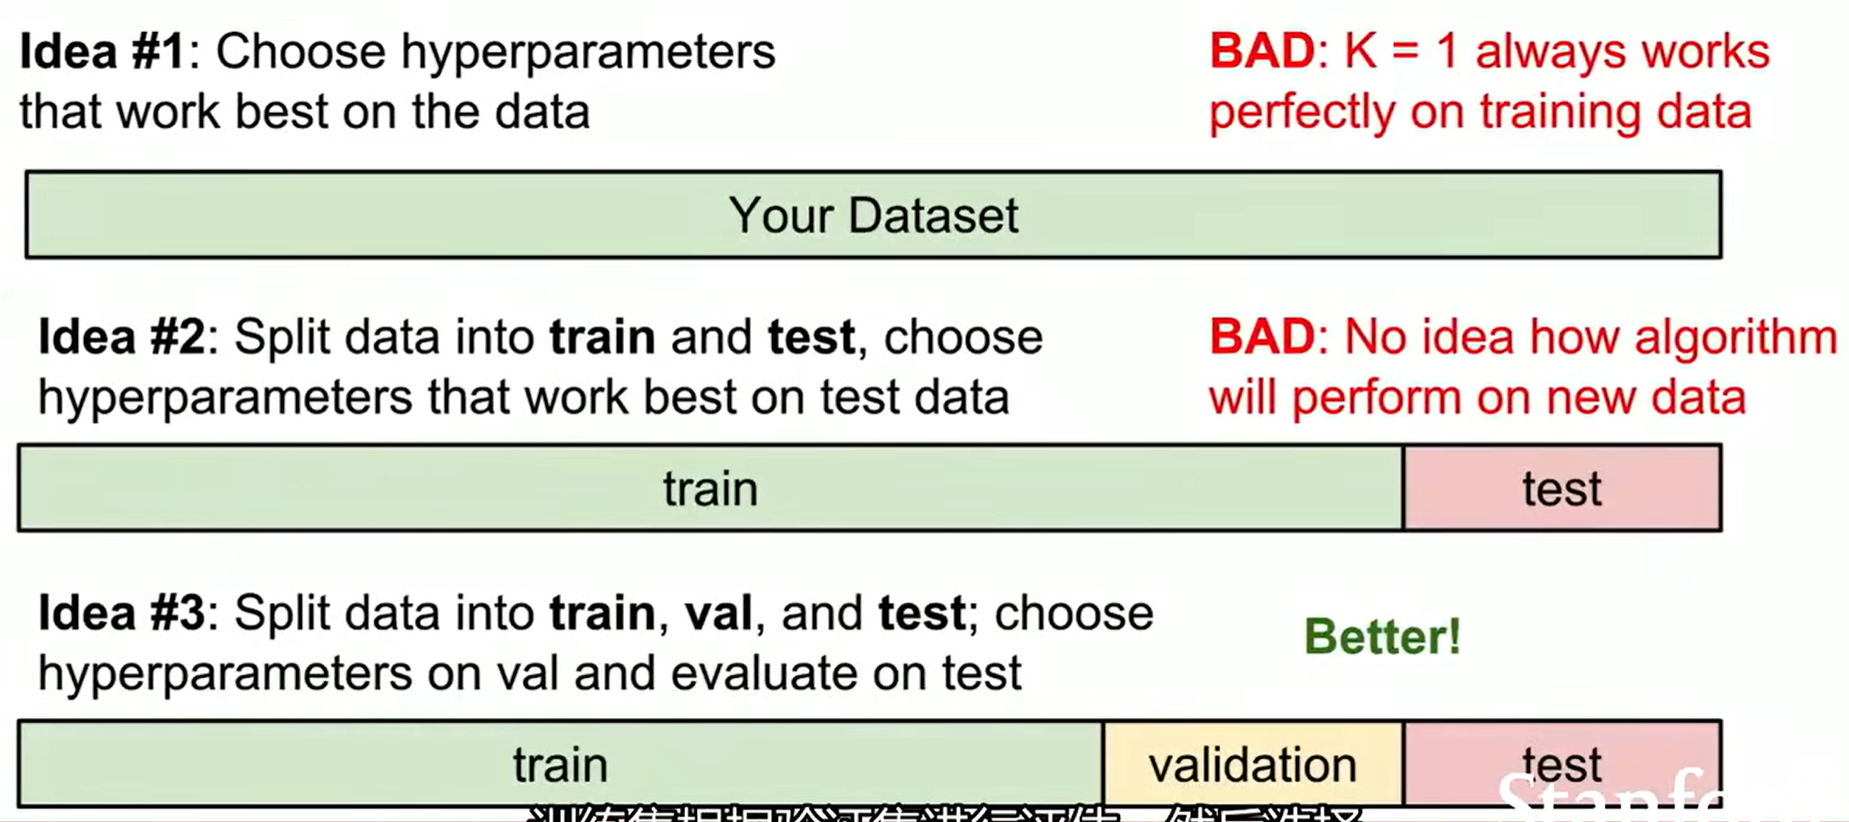
\includegraphics[width=0.8\textwidth]{images/Lecture1/ideas_for_hyperparameter.png}
                \item \textbf{The common idea:} Cross-validation(交叉验证).\par
                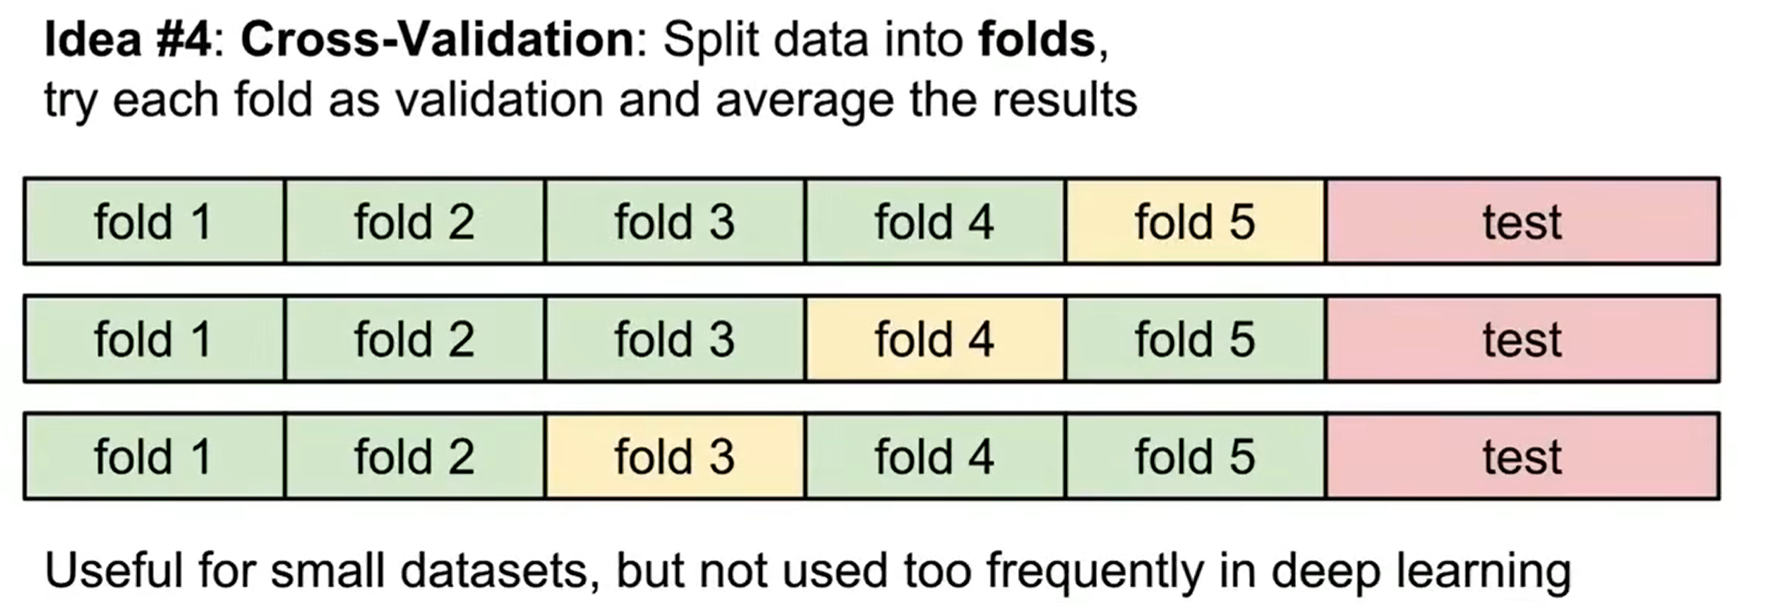
\includegraphics[width=0.8\textwidth]{images/Lecture1/cross_validation.png}
            \end{itemize}

            \item \textit{Pros and Cons:}\par
            Actually, KNN on image is never used:\par
            - Very slow at test time.\par
            - Distance-metrics on pixels are not informative.\par
            - Curse of dimensionality: as the number of dimensions increases, the distance between points becomes less meaningful.\par
        \end{itemize}

        \item \textbf{Linear Classifier:}
        \begin{itemize}
            \item \textit{Description:} A linear classifier makes its predictions based on a linear predictor function combining a set of weights with the feature vector.\par
            \begin{equation}
                f(x, W) = Wx + b
            \end{equation}
            where \(x\) is the input image and \(w\) is the weight vector, \(b\) is the bias term.\par
            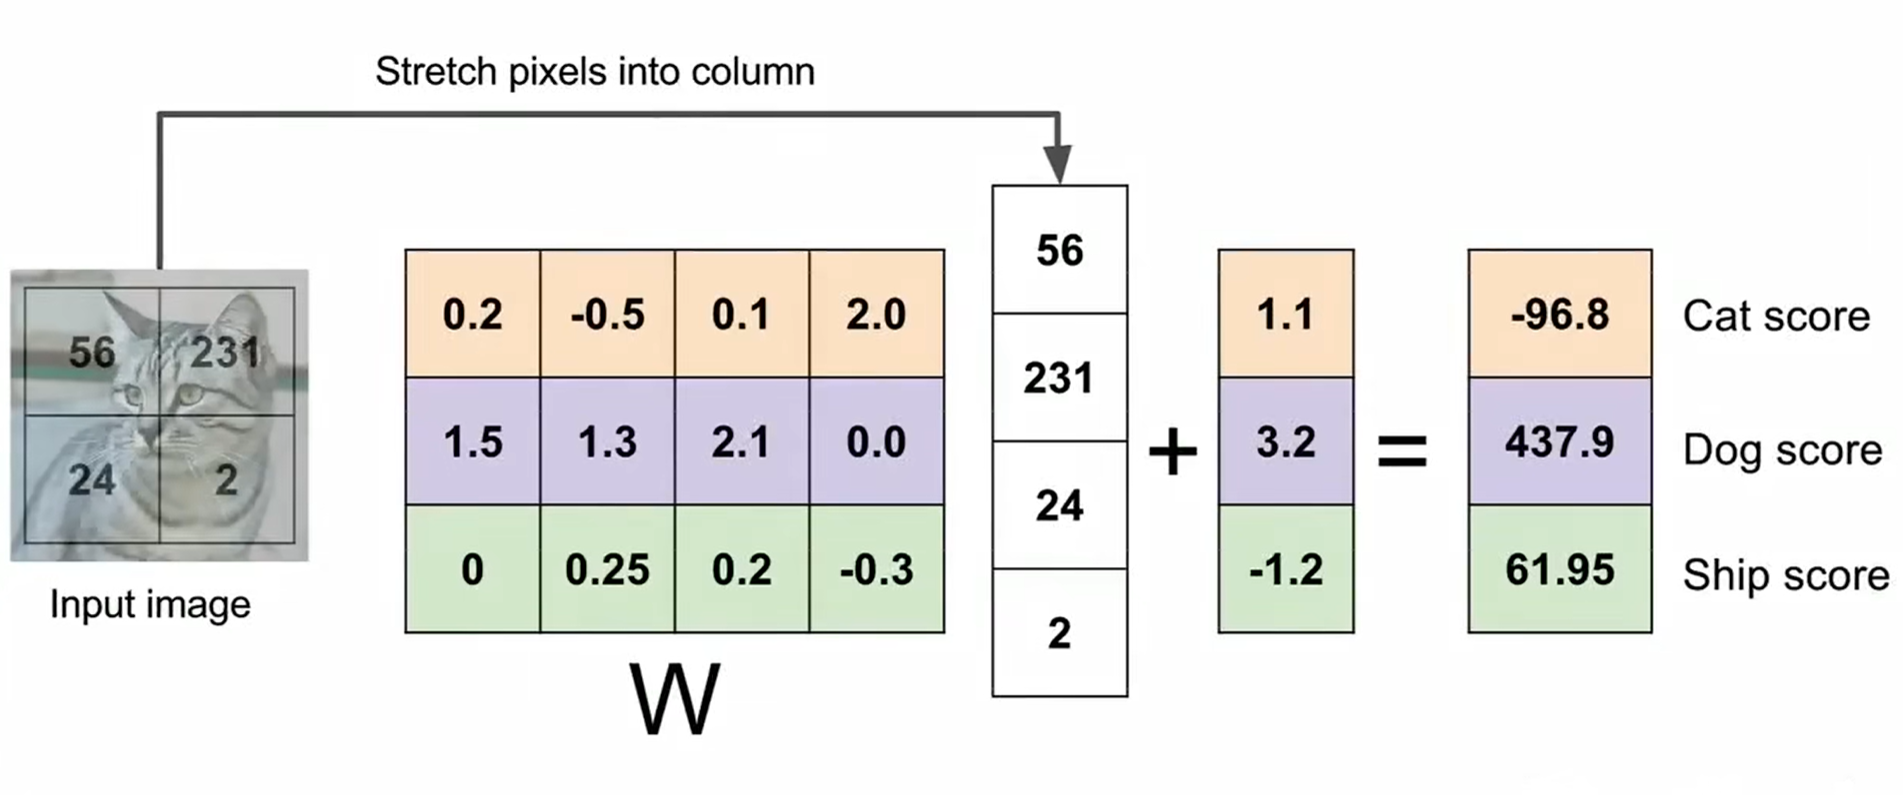
\includegraphics[width=0.8\textwidth]{images/Lecture1/linear_classifier_example.png}
            \item \textit{Hard cases:}\par
            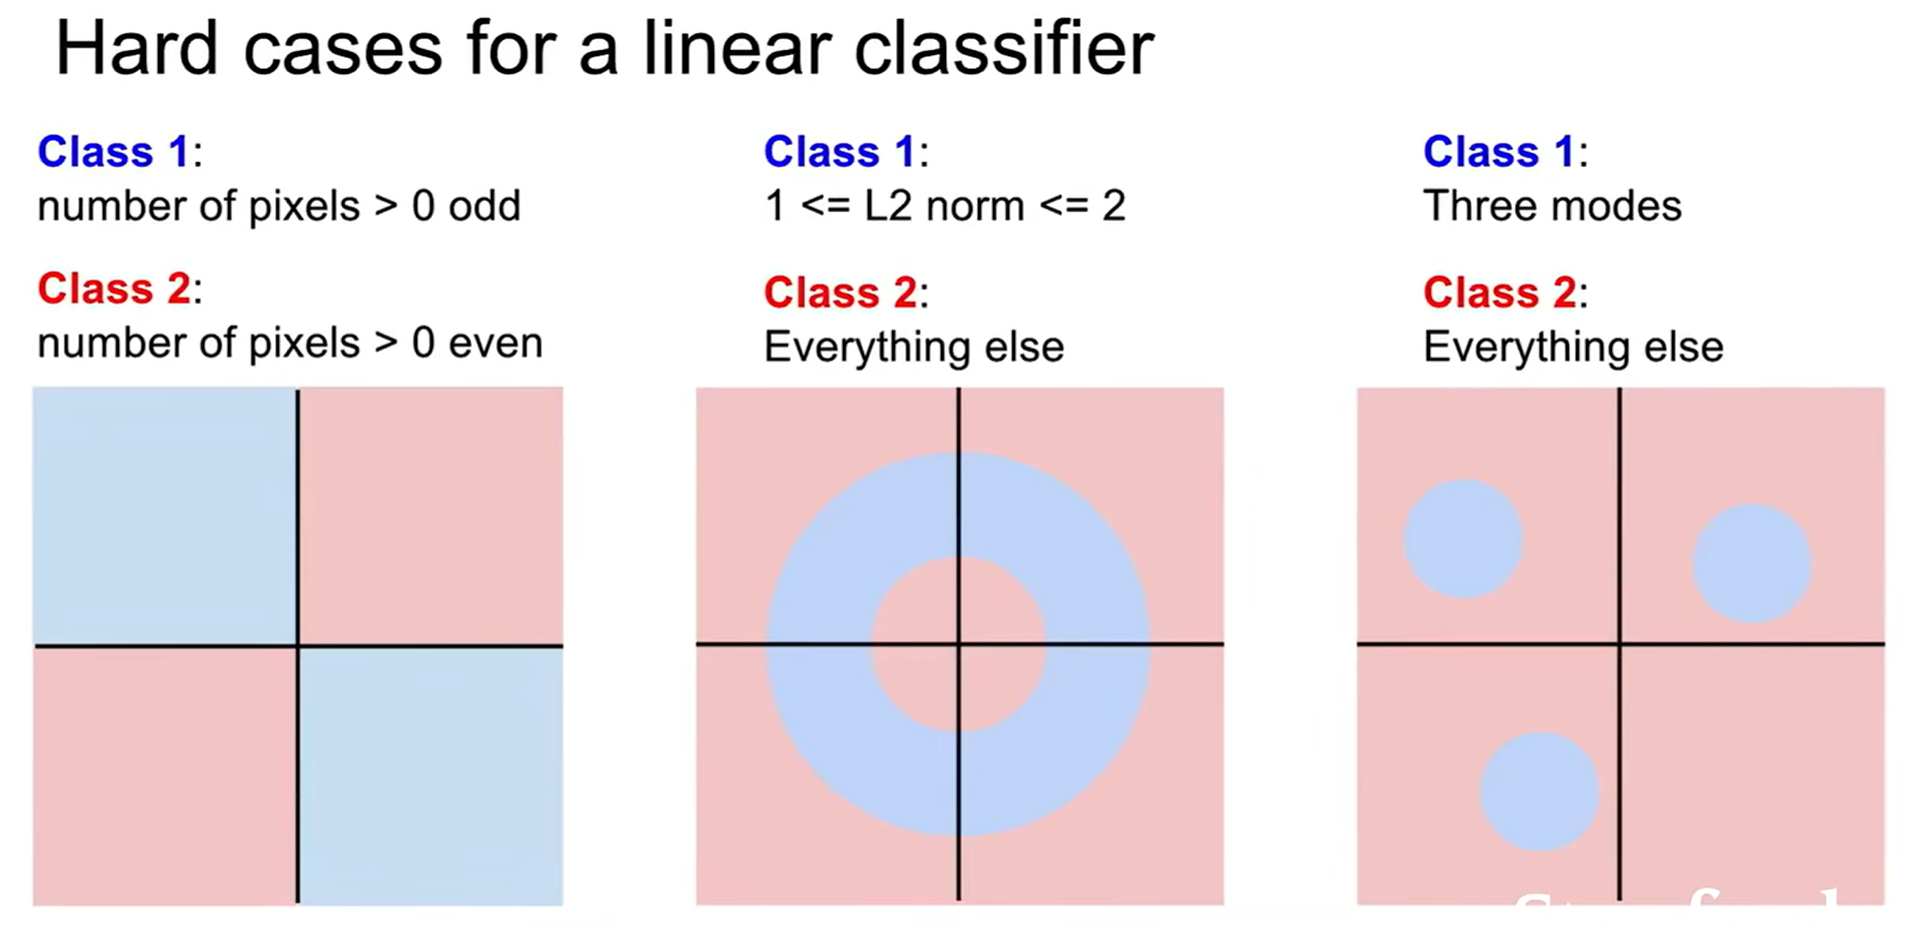
\includegraphics[width=0.8\textwidth]{images/Lecture1/hard_cases_for_linear_classifier.png}
        \end{itemize}


    \end{enumerate}
\end{enumerate}

\end{CJK}
\end{document}




